\documentclass{article} % Tipo de documento

\usepackage[utf8]{inputenc} % Permite el uso de caracteres del Español

\usepackage[T1]{fontenc}

\usepackage{graphicx}

\usepackage{subfig}

% Carátula del Artículo  

\title{Evaluación 1}

\author{Brenda Leyva Amaya}

\date{8 de Marzo, 2018}
 

\begin{document}

\maketitle % Crea el título

 \begin{center}
 	
\includegraphics[width=9cm]{examen.jpg}
 \end{center}

\section{Archivos de datos.}

Se han decargado dos archivos que guardan datos de las distintas tomas del equipo en la estación, uno de ellos es referente a la salinidad y el otro contiene datos más generales de la zona. 

\vspace{0.5 cm}

Los archivos tienen la misma estructura de columnas y los datos corresponden a tomas cada 15 minutos con su fecha correspondiente. Estos archivos se han proporcionado de manera que pueden ser leídos por jupyter. No ha sido necesario llevar a cabo una limpieza de los mismos. 

\vspace{0.5 cm}

De manera que se procede directamente a leerlos y crear los correpondientes data frames.


\section{Uso de Jupyter Notebook.}

Utilizamos Jupyter Notebook para llevar a cabo análisis de los datos. A continuación se describen y muestras las actividades que se llevaron a cabo. Primero que nada se ha hecho la lectura de los archivos en jupyter y después se comenzó el análisis de datos. 

 \begin{center}
 	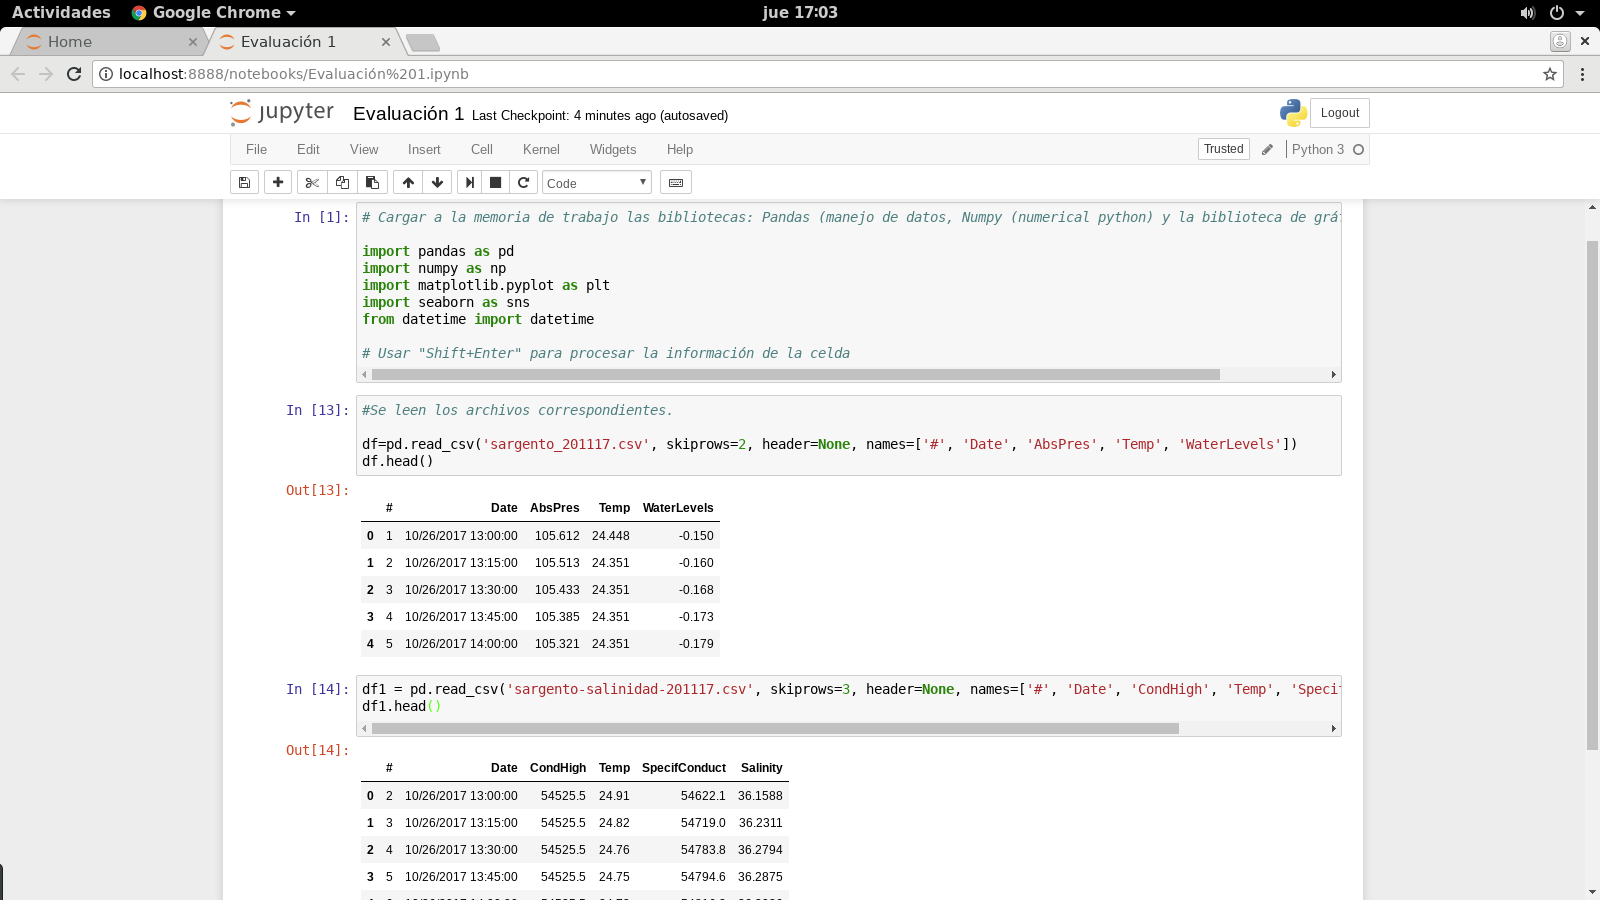
\includegraphics[width=12cm]{lectura.png}
 \end{center}

\subsection{Biblioteca Seaborn.}

El primer paso será abordar la herramienta Seaborn para crear gráficos y ejercicios correspondientes. 

\subsubsection{Gráficas de caja.}

\hspace{0.45 cm}a) Nivel de mar (metros)

\begin{verbatim} 

box1 = sns.boxplot(x="month", y="WaterLevels", data=df)
plt.show()

\end{verbatim}


 \begin{center}
 	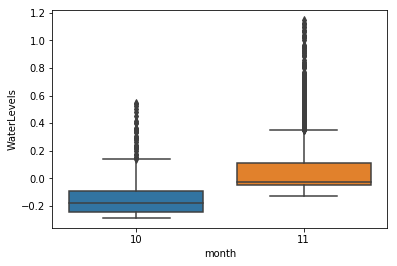
\includegraphics[width=10cm]{box1.png}
 \end{center}


b) Salinidad (Partes por mil - ppt)


\begin{verbatim} 

box2 = sns.boxplot(x="month", y="Salinity", data=df1)
plt.show()

\end{verbatim}


 \begin{center}
 	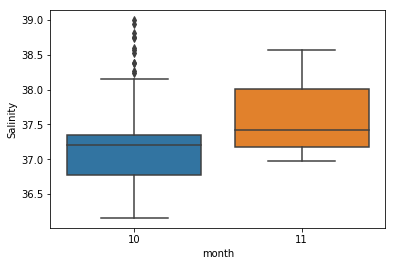
\includegraphics[width=10cm]{box2.png}
 \end{center}
 

c) Temperatura de Agua (ºC).

\begin{verbatim} 

box3 = sns.boxplot(x="month", y="Temp", data=df1)
plt.show()

\end{verbatim}

 \begin{center}
 	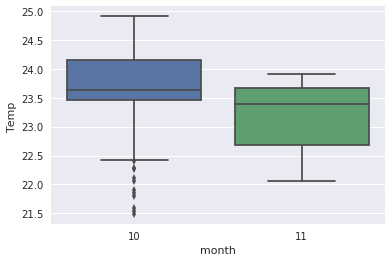
\includegraphics[width=10cm]{box3.png}
 \end{center}
 
 
\subsubsection{Función "Describe".}

A continuación se presenta el análisis estadístico con el uso de la función describe.


 \begin{center}
 	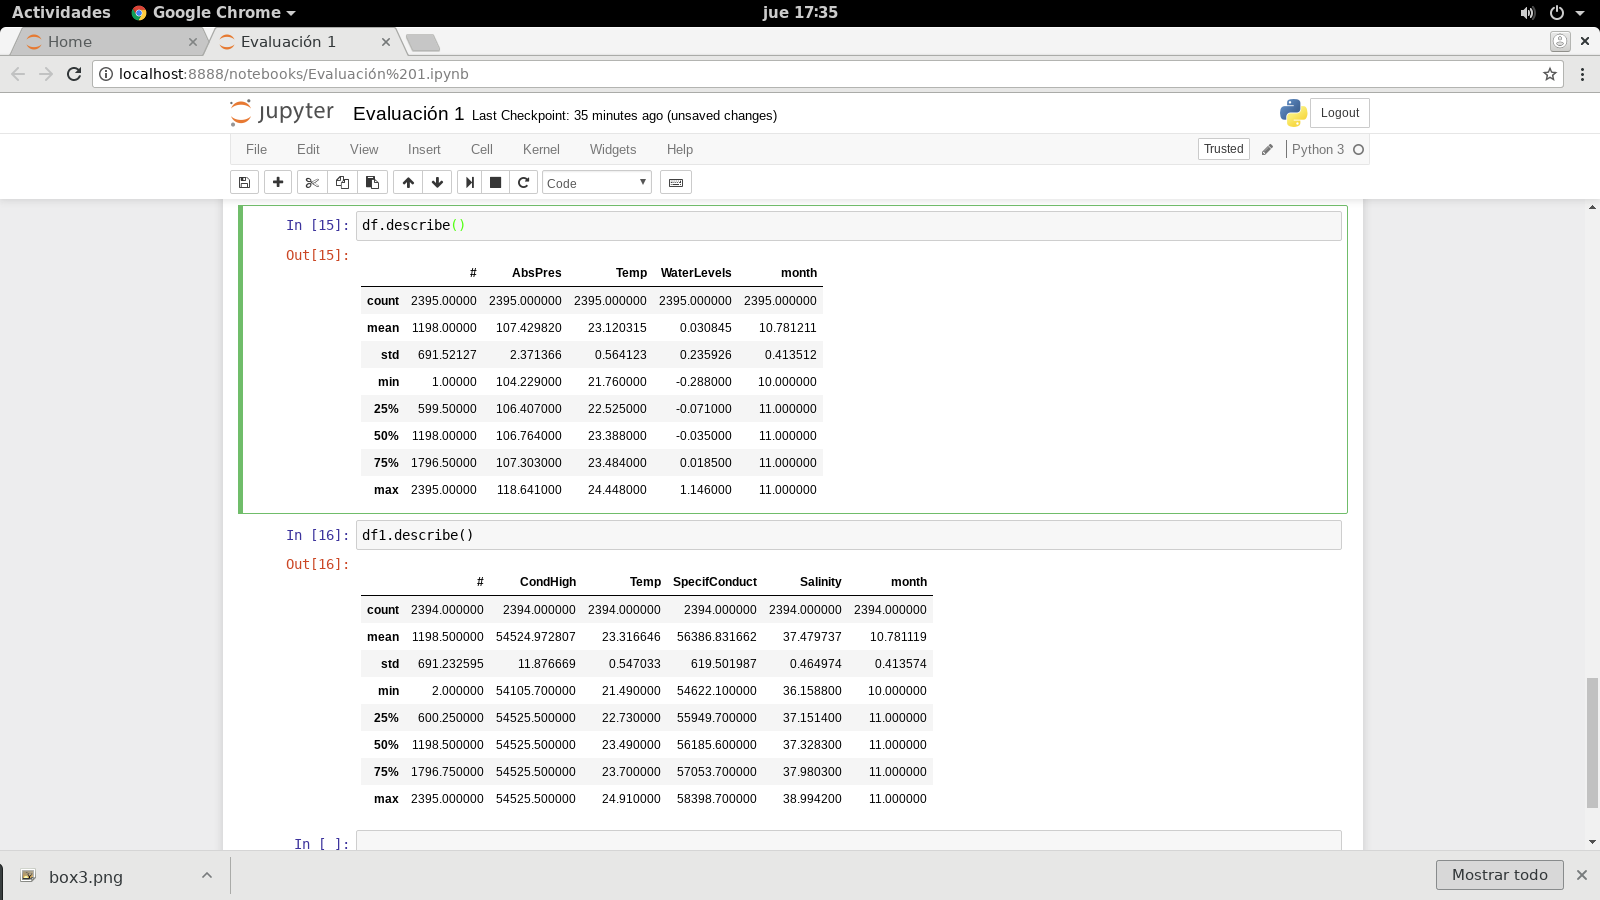
\includegraphics[width=10cm]{describe.png}
 \end{center}


\subsubsection{Correlaciones.}

\hspace{0.45 cm}Nivel de mar-Salinidad.

\begin{verbatim} 

sns.set(style="darkgrid", color_codes=True)

ws = sns.jointplot("WaterLevels", "Salinity", data=pd.concat([df,df1],axis=1,join_axes=[df1.index]), kind="reg",color="r", size=7)
plt.show(ws)

\end{verbatim}

 \begin{center}
 	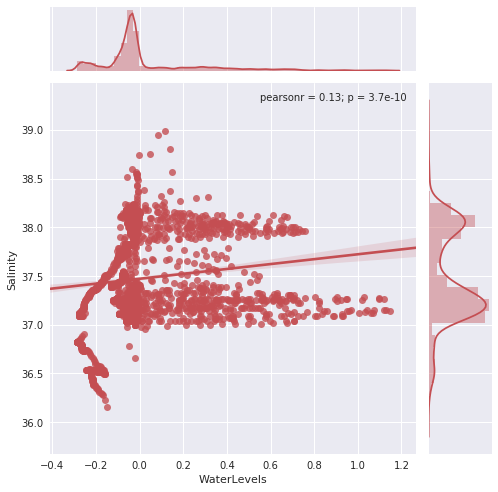
\includegraphics[width=7cm]{ws.png}
 \end{center}

Nivel de mar-Temperatura del agua.

\begin{verbatim} 

sns.set(style="darkgrid", color_codes=True)

wt = sns.jointplot("WaterLevels", "Temp", data=df, kind="reg",color="r", size=7)
plt.show(wt)

\end{verbatim}


 \begin{center}
 	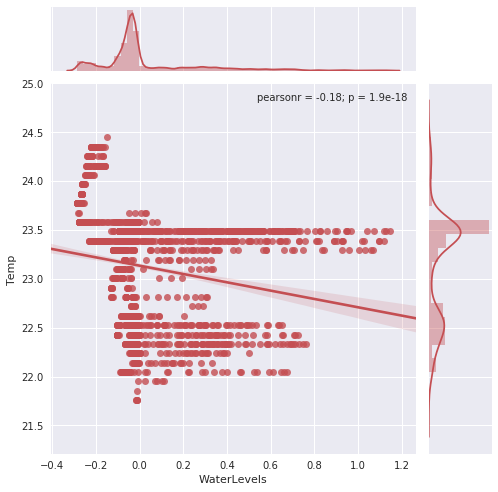
\includegraphics[width=12cm]{wt.png}
 \end{center}


Salinidad-Temperatura del agua. 

\begin{verbatim} 

sns.set(style="darkgrid", color_codes=True)

st = sns.jointplot("Salinity", "Temp", data=df1, kind="reg",color="r", size=7)
plt.show(st)

\end{verbatim}

 \begin{center}
 	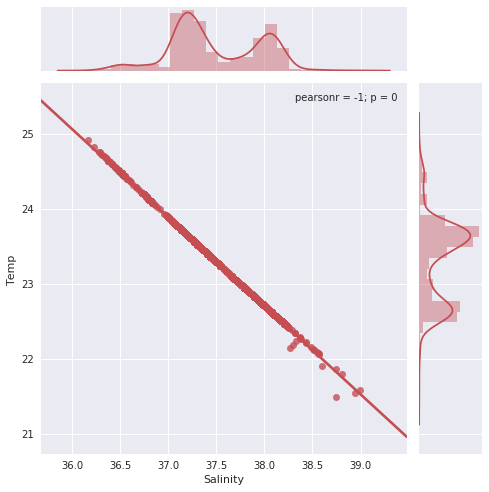
\includegraphics[width=12cm]{st.png}
 \end{center}
 

\subsection{Matplotlib.}

A continuación utilizaremos la herramienta Matplotlib para realizar las siguientes actividades. 

\subsubsection{Variables VS tiempo.}

\hspace{0.45 cm}Nivel del mar

\begin{verbatim} 

plt.plot_date(x=df.Ndate, y=df.WaterLevels, fmt="b-")
plt.title("Variación de los niveles de agua")
plt.ylabel("Niveles de agua")
plt.grid(True)
plt.show()

\end{verbatim}


\begin{center}
 	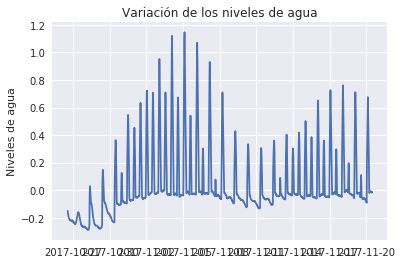
\includegraphics[width=11cm]{wat.png}
 \end{center}

Salinidad

\begin{verbatim} 

plt.plot_date(x=df1.Ndate, y=df1.Salinity, fmt="b-")
plt.title("Variación de la salinidad")
plt.ylabel("Salinidad")
plt.grid(True)
plt.show()

\end{verbatim}

\begin{center}
 	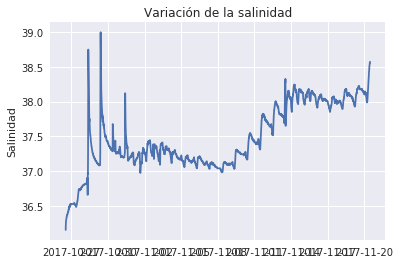
\includegraphics[width=11cm]{salit.png}
 \end{center}

Temperatura del Agua

\begin{verbatim} 

plt.plot_date(x=df1.Ndate, y=df1.Temp, fmt="b-")
plt.title("Variación en la temperatura")
plt.ylabel("Temperatura")
plt.grid(True)
plt.show()

\end{verbatim}

\begin{center}
 	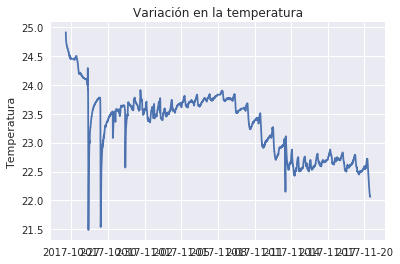
\includegraphics[width=11cm]{tempt.png}
 \end{center}


\subsubsection{Gráficas superpuestas.}

\hspace{0.45 cm} a) Nivel de mar y Salinidad


\begin{verbatim} 

from matplotlib import rc
rc('mathtext', default='regular')

df2 = pd.concat([df.WaterLevels, df1.Salinity],axis=1)

fig = plt.figure()
ax = fig.add_subplot(111)

Fecha=df.Ndate
WL=df.WaterLevels
SAL=df1.Salinity

ax.plot(Fecha, WL, '-b', label = 'Nivel de agua')

ax2 = ax.twinx()
ax2.plot(Fecha, SAL, '-r', label = 'Salinidad')

ax.legend(loc=0)
ax.grid()

plt.show()

\end{verbatim}


\begin{center}
 	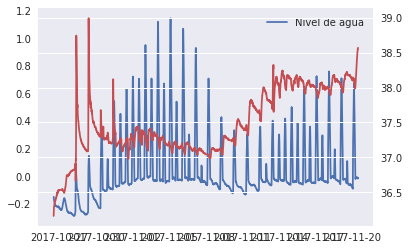
\includegraphics[width=11cm]{sobre1.png}
\end{center}


b) Nivel de mar y Temperatura.

\begin{verbatim} 

from matplotlib import rc
rc('mathtext', default='regular')

fig = plt.figure()
ax = fig.add_subplot(111)

Fecha=df.Ndate
WL=df.WaterLevels
Temp=df.Temp

ax.plot(Fecha, WL, '-b', label = 'Nivel de agua')

ax2 = ax.twinx()
ax2.plot(Fecha, Temp, '-r', label = 'Temperatura')

ax.legend(loc=0)
ax.grid()

plt.show()

\end{verbatim}


\begin{center}
 	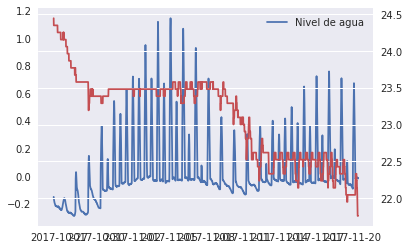
\includegraphics[width=11cm]{sobre2.png}
\end{center}


Para 5 días:

a) Nivel de mar y Salinidad

\begin{verbatim} 

from matplotlib import rc
rc('mathtext', default='regular')

df2 = pd.concat([df.WaterLevels, df1.Salinity],axis=1)

fig = plt.figure()
ax = fig.add_subplot(111)

Fecha=df.Ndate
WL=df.WaterLevels
SAL=df1.Salinity

ax.plot(Fecha, WL, '-b', label = 'Nivel de agua')

ax2 = ax.twinx()
ax2.plot(Fecha, SAL, '-r', label = 'Salinidad')

ax2.set_xlim("10/26/2017 13:00:00","10/27/2017 00:00:00")
ax.set_xlim("10/26/2017 13:00:00","10/27/2017 00:00:00")


ax.legend(loc=0)
ax.grid()

plt.show()
\end{verbatim}

\begin{center}
 	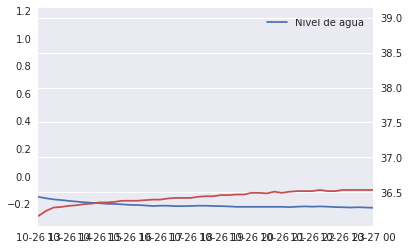
\includegraphics[width=11cm]{5dias1.png}
\end{center}


b) Nivel de mar y Temperatura.

\begin{verbatim} 

from matplotlib import rc
rc('mathtext', default='regular')

fig = plt.figure()
ax = fig.add_subplot(111)

Fecha=df.Ndate
WL=df.WaterLevels
Temp=df.Temp

ax.plot(Fecha, WL, '-b', label = 'Nivel de agua')

ax2 = ax.twinx()
ax2.plot(Fecha, Temp, '-r', label = 'Temperatura')

ax2.set_xlim("10/26/2017 13:00:00","10/27/2017 00:00:00")
ax.set_xlim("10/26/2017 13:00:00","10/27/2017 00:00:00")

ax.legend(loc=0)
ax.grid()

plt.show()
\end{verbatim}


\begin{center}
 	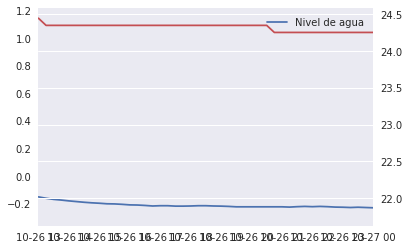
\includegraphics[width=11cm]{5dias2.png}
\end{center}

\section{Conclusiones.}

La actividad se llevó a cabo satisfactoriamente, se encontraron datos interesantes sobre todo en la correlación de la salinidad del agua con su temperatura pues esta se observó en su comportamiento gráfico como una relación casi perfectamente lineal, con muy pocos datos fuera de la interpolación. Se espera que las actividades realizadas se hayan llevado a cabo de manera correcta y que cumplan las metas fijadas para la evaluación. 

\end{document}